%%____________________________________________________________________________||
\section{Trigger strategy}
\label{sec:triggers}


\subsection{Hadronic signal region}

In Run 2 the RA1 analysis will aim to retain the low-thresholds of Run 1 with developments to the trigger selection, maintaining sensitivity to signatures of new physics with hadronic energies as low as $\scalht = 200$ GeV. This in part is achieved by a migration to PF-based jet reconstruction within the HLT which, in conjunction with a reduction of clustering radius parameter $\Delta R = 0.4$, provides improvements in jet energy resolution in high-pileup conditions and mitigates the effects of pileup contamination within the jet cone.

A suite of $\scalht$-$\alphat$ cross-triggers with a requirement on the minimum average \pt of the leading two jets, $\pt^{\rm \left<j1,j2\right>$, are utilised in the selection of events in the hadronic signal region, labelled: \verb!HLT_PFHTXXX_PFDijetYYY_AlphaT0pZZ!. The use of a dijet average threshold provides an improved suppression of QCD multijet events enabling the use of looser \alphaT thresholds whilst maintaining acceptance to events exhibiting asymmetric jet topologies such as monojet-like signatures of compressed spectrum and DM models. A loose calorimeter trigger prefilter is utilised to reduce the pass-through rate prior to track-based reconstruction, ensuring the PF-based filters meet timing requirements. The calorimeter prefilter utilises loose \scalht and dijet average \pt requirements in addition to a new variable \alphat', defined as \alphat in the limit $\Delta\scalht \rightarrow 0$, which better correlates \alphat between calorimeter and PF-based reconstruction.

The thresholds of the signal triggers, shown in Table~\ref{tab:2015_Hadronic_Signal_Triggers}, are tuned to maintain acceptance to a range of signal topologies whilst effectively suppressing QCD multijet events to maintain acceptable trigger rates. These uniquely seed individual offline \scalht bins with the exception of the highest-\scalht trigger which is utilised for analysis bins in the range: $400 < \scalht < 800$ \GeV. Above $\scalht > 800$ a pure \scalht trigger, \verb!HLT_PFHT800!, is utilised which has no explicit dependence on $\alphat$ or dijet average threshold. In addition to the primary triggers, a set of backup triggers with higher thresholds are utilised to provide protection for higher luminosity scenarios. The Level-1 seeds for the HLT paths are given by the disjunction of the lowest unprescaled Level-1 hadronic scalar energy and missing energy sum seeds (\verb!HTTXXX_OR_ETMYYY!) for the given run scenario.


% TABLE : 2015 triggers
%----------------------------------------------------------------------
\begin{table}[h!]
\topcaption{Trigger thresholds of the Level-1, calorimeter prefilter and final PF-trigger decision for the primary HLT paths for the hadronic signal region in the $\lumi=1.4\times10^{34}$ PU40bx25 scenario. Lower threshold Level-1 \scalht and \met seeds are utilised for the lower luminosity scenarios. }
\footnotesize
\centering
%\begin{tabular}{c|ccc|c} 
\begin{tabular}{c|ccc} 
\hline
\hline
HLT path & L1 seed & HLT calo-prefilter                      & HLT PF-filter                          \\ %& Rate \\[0.7 ex] 
         &         & ($\scalht$, $\alphat$', $\pt^{\rm \left<j1,j2\right>$) & ($\scalht$, $\alphat$, $\pt^{\rm \left<j1,j2\right>$) \\ %& (Hz) \\[0.7 ex] 
\hline
\verb!HLT_PFHT200_PFDijetAve90_AlphaT0p57! & \verb!HTT175 OR ETM70! & 150, 0.540, 70 & 200, 0.570, 90 \\ %& \\ % 11.0 $\pm$ 3.0 \\
\verb!HLT_PFHT250_PFDijetAve90_AlphaT0p55! & \verb!HTT175 OR ETM70! & 200, 0.535, 70 & 250, 0.550, 90 \\ %& \\ % 8.5  $\pm$ 3.0 \\
\verb!HLT_PFHT300_PFDijetAve90_AlphaT0p53! & \verb!HTT175 OR ETM70! & 250, 0.525, 70 & 300, 0.530, 90 \\ %& \\ % 9.5  $\pm$ 3.0 \\
\verb!HLT_PFHT350_PFDijetAve90_AlphaT0p52! & \verb!HTT175 OR ETM70! & 300, 0.520, 70 & 350, 0.520, 90 \\ %& \\ % 10.0 $\pm$ 3.0 \\
\verb!HLT_PFHT400_PFDijetAve90_AlphaT0p51! & \verb!HTT175 OR ETM70! & 370, 0.510, 70 & 400, 0.510, 90 \\ %& \\ % 13.5 $\pm$ 3.5 \\ \\ %\hline \\ %\multicolumn{4}{c|}{Exclusive rate (Hz)} & \\ % 34 $\pm$ 6 \\
\hline
\hline

\end{tabular}
\label{tab:2015_Hadronic_Signal_Triggers}
\end{table}




The Measurement of trigger efficiency in data with an orthogonal \verb!SingleMu! dataset, seeded by the \verb!HLT_IsoMu24_eta2p1! trigger.
Selection of sample: $|\eta| < 2.1$

The muon is excluded in the computation of event variables.



The trigger efficiency measured for a signal model is shown in Figure~\ref{fig:T1ttt_Trigger_Efficiency}




% FIGURE: Trigger efficiencies
%----------------------------------------------------------------------
\begin{figure}[h!]
  \begin{center}
    \subfigure[$\njet = 4$]   {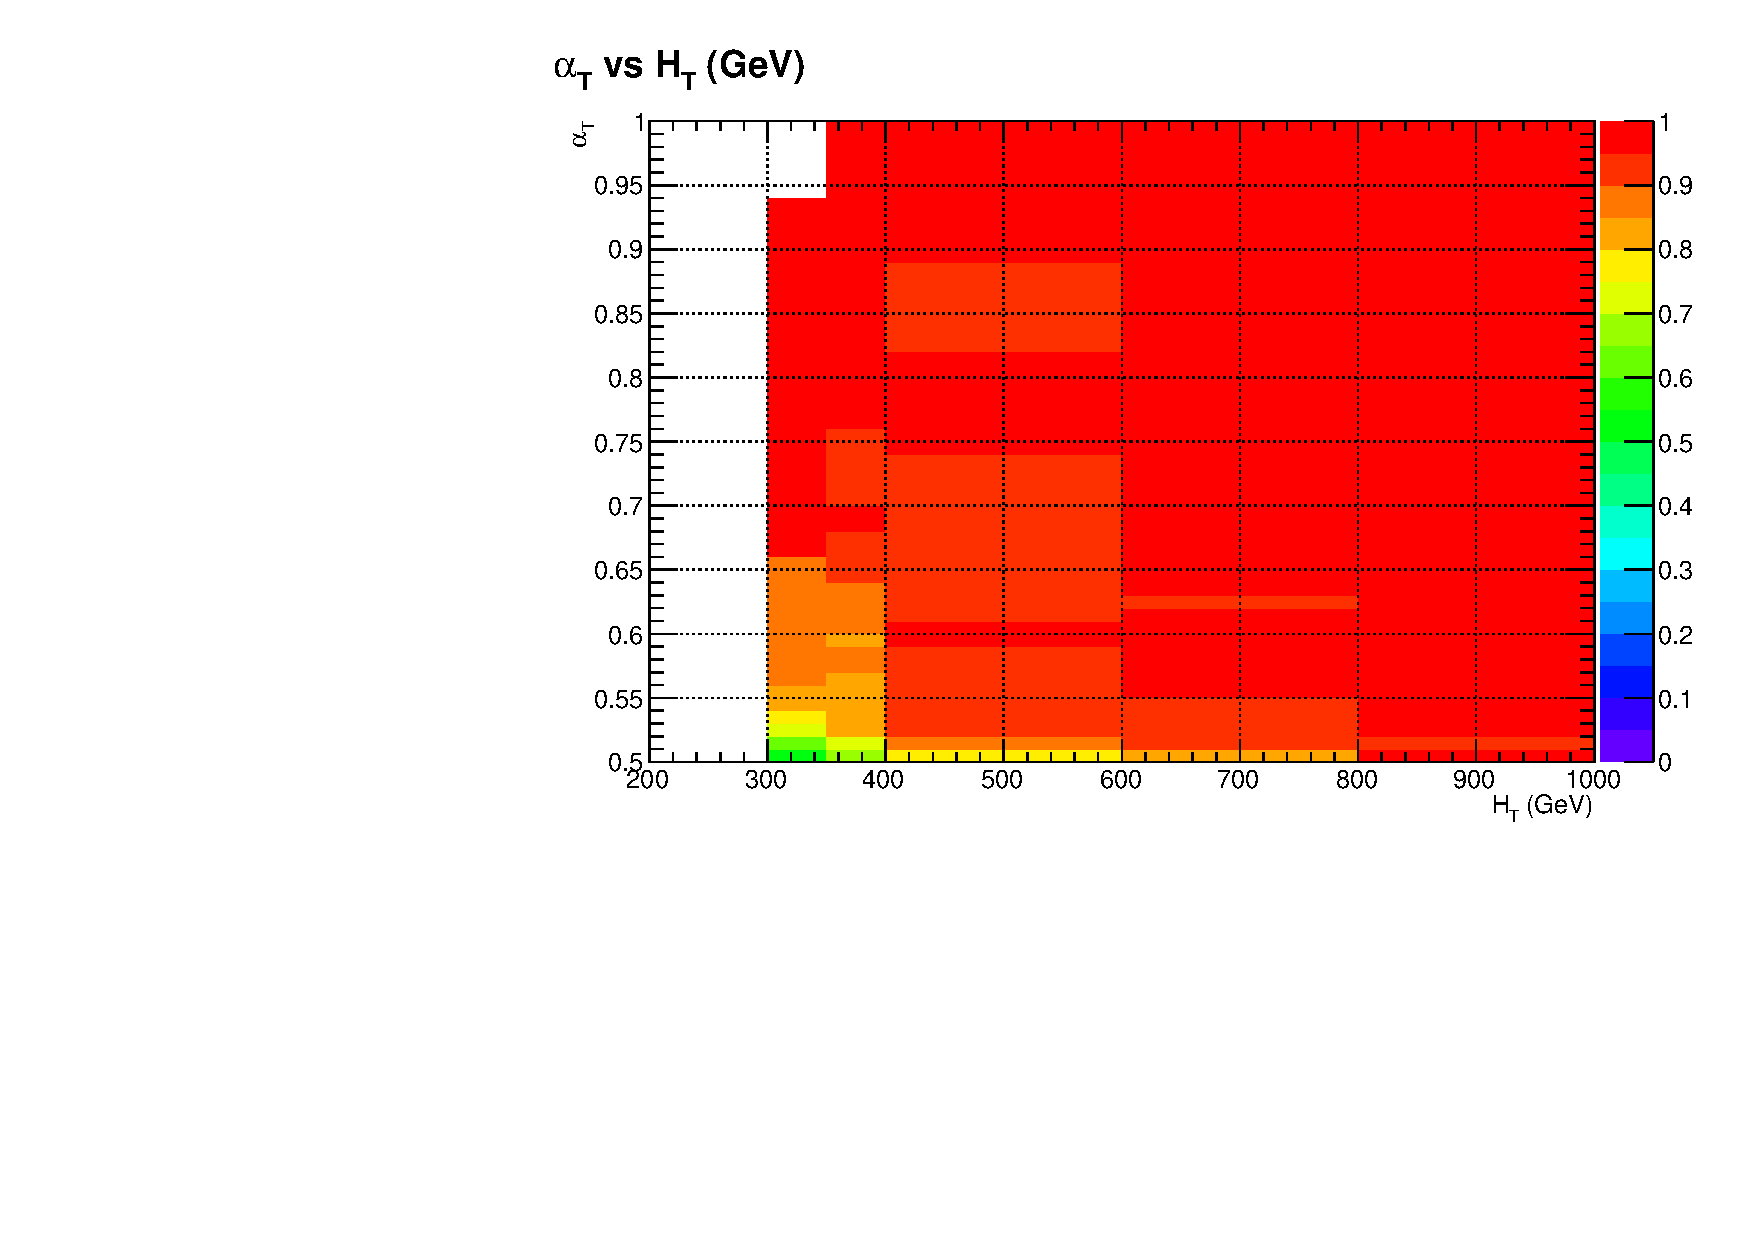
\includegraphics[width=0.5\textwidth]{figures/Trigger/eq4j_ht_vs_alphaT_Cumul.pdf}} ~~
    \subfigure[$\njet \geq 5$]{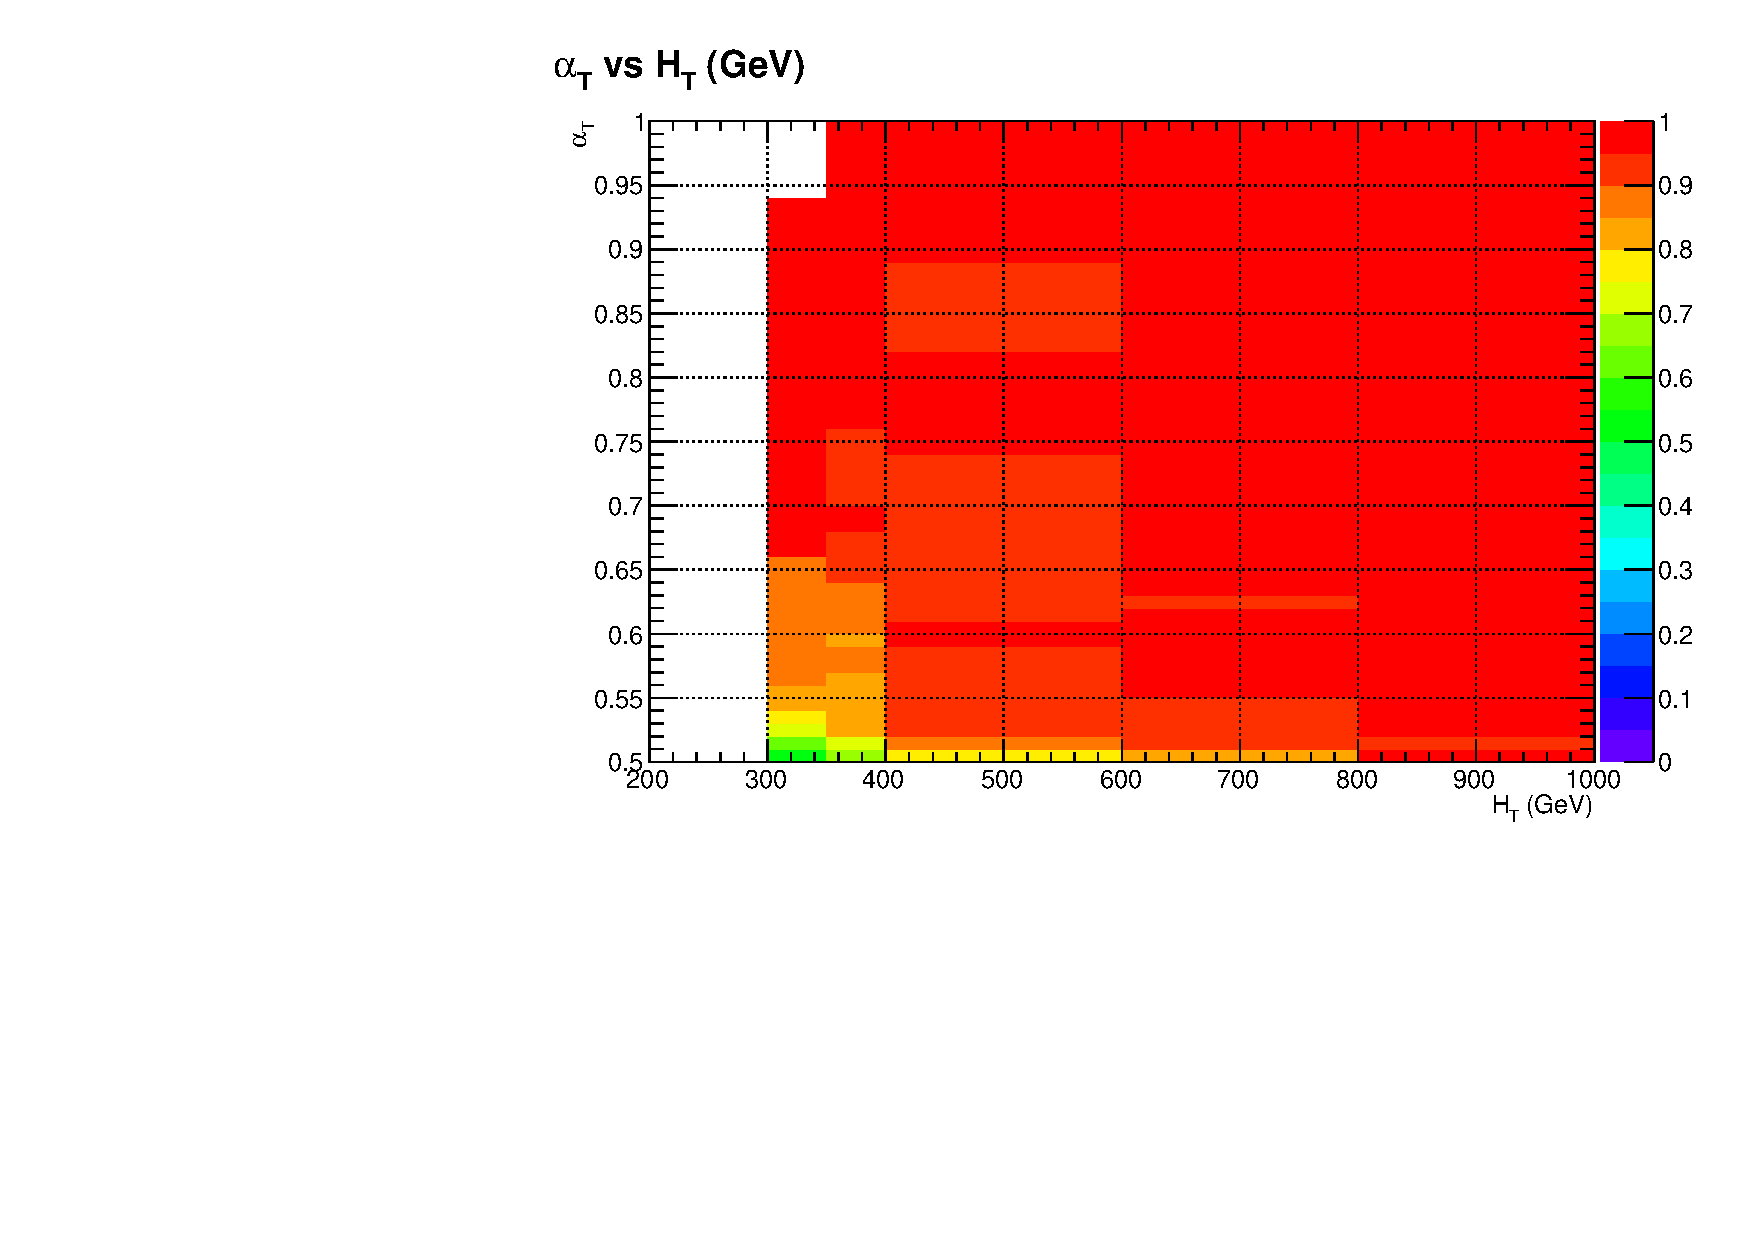
\includegraphics[width=0.5\textwidth]{figures/Trigger/eq4j_ht_vs_alphaT_Cumul.pdf}} \\
    \subfigure[$\njet = 4$]   {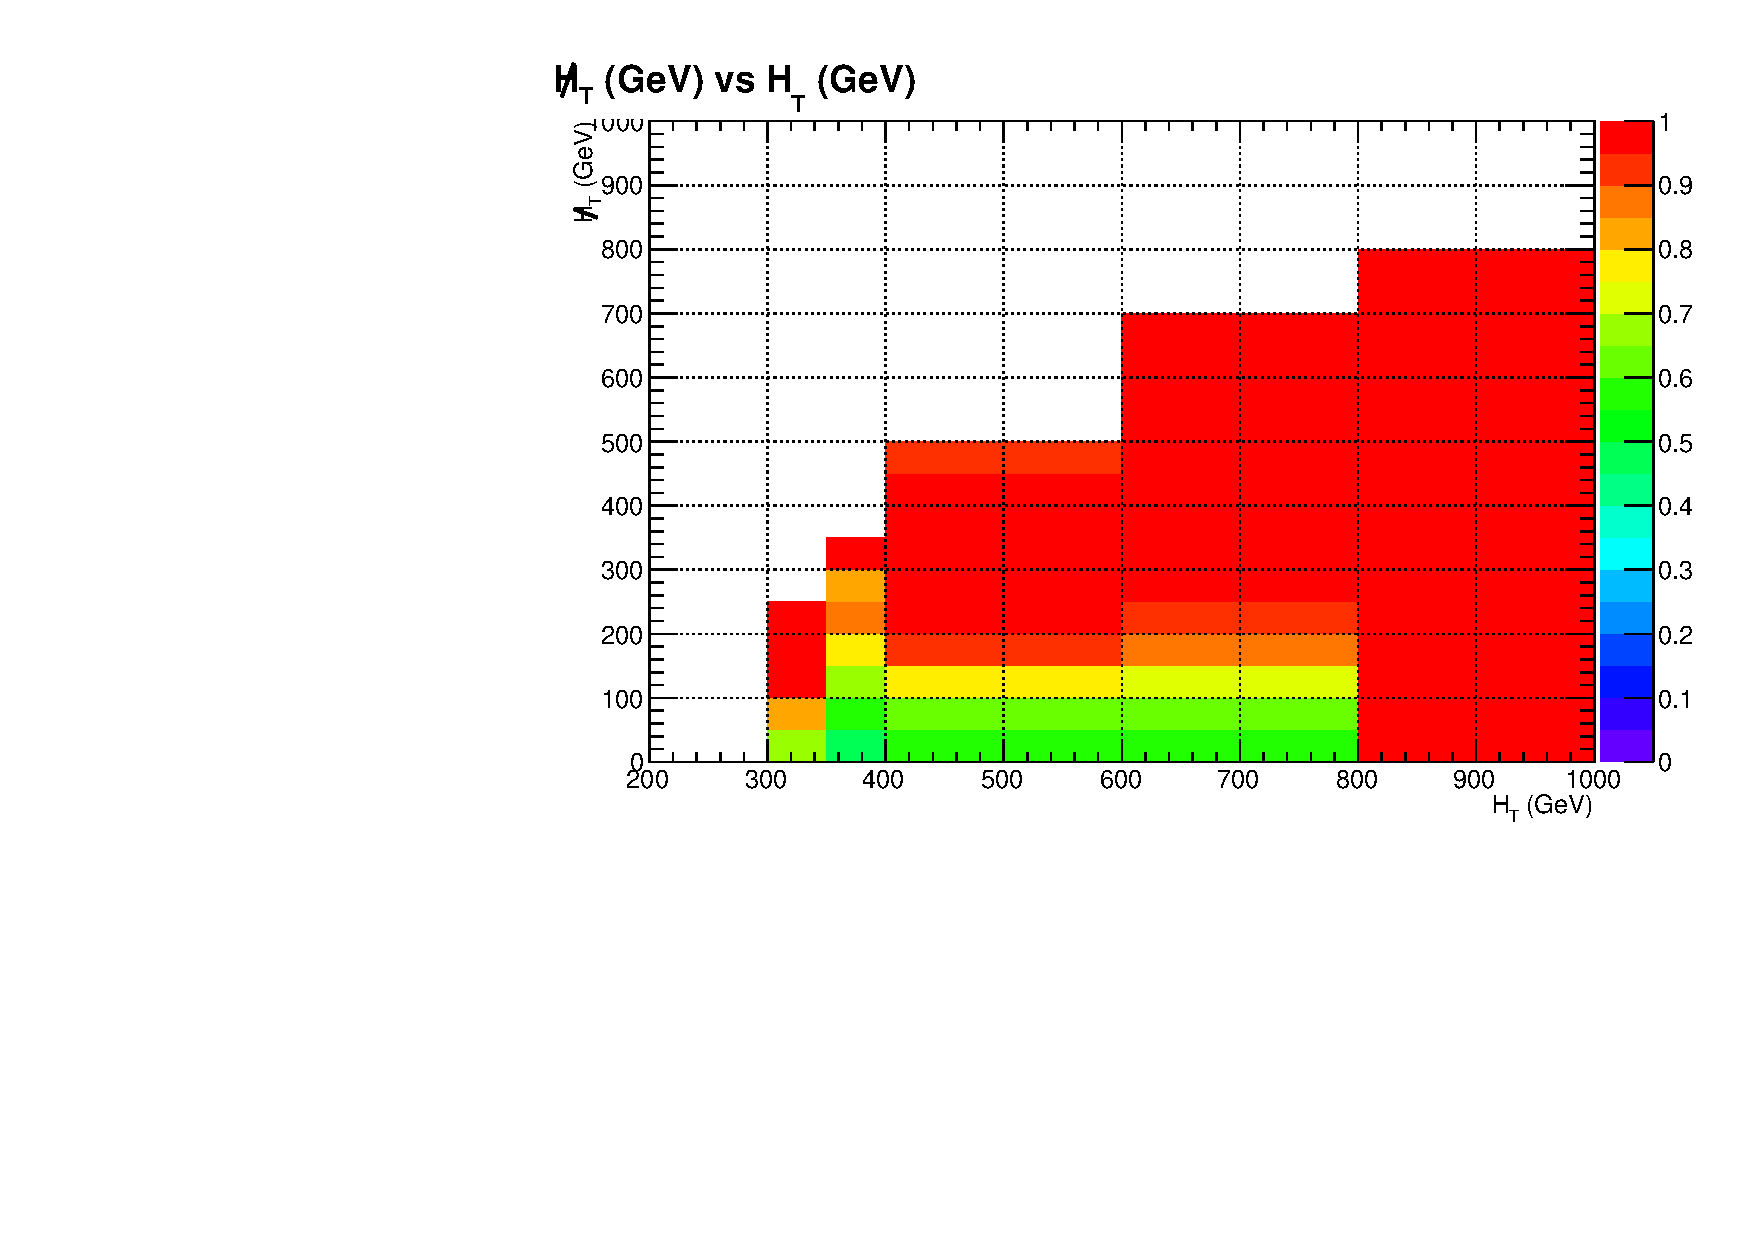
\includegraphics[width=0.5\textwidth]{figures/Trigger/ge5j_ht_vs_mht_Cumul.pdf}} ~~
    \subfigure[$\njet \geq 5$]{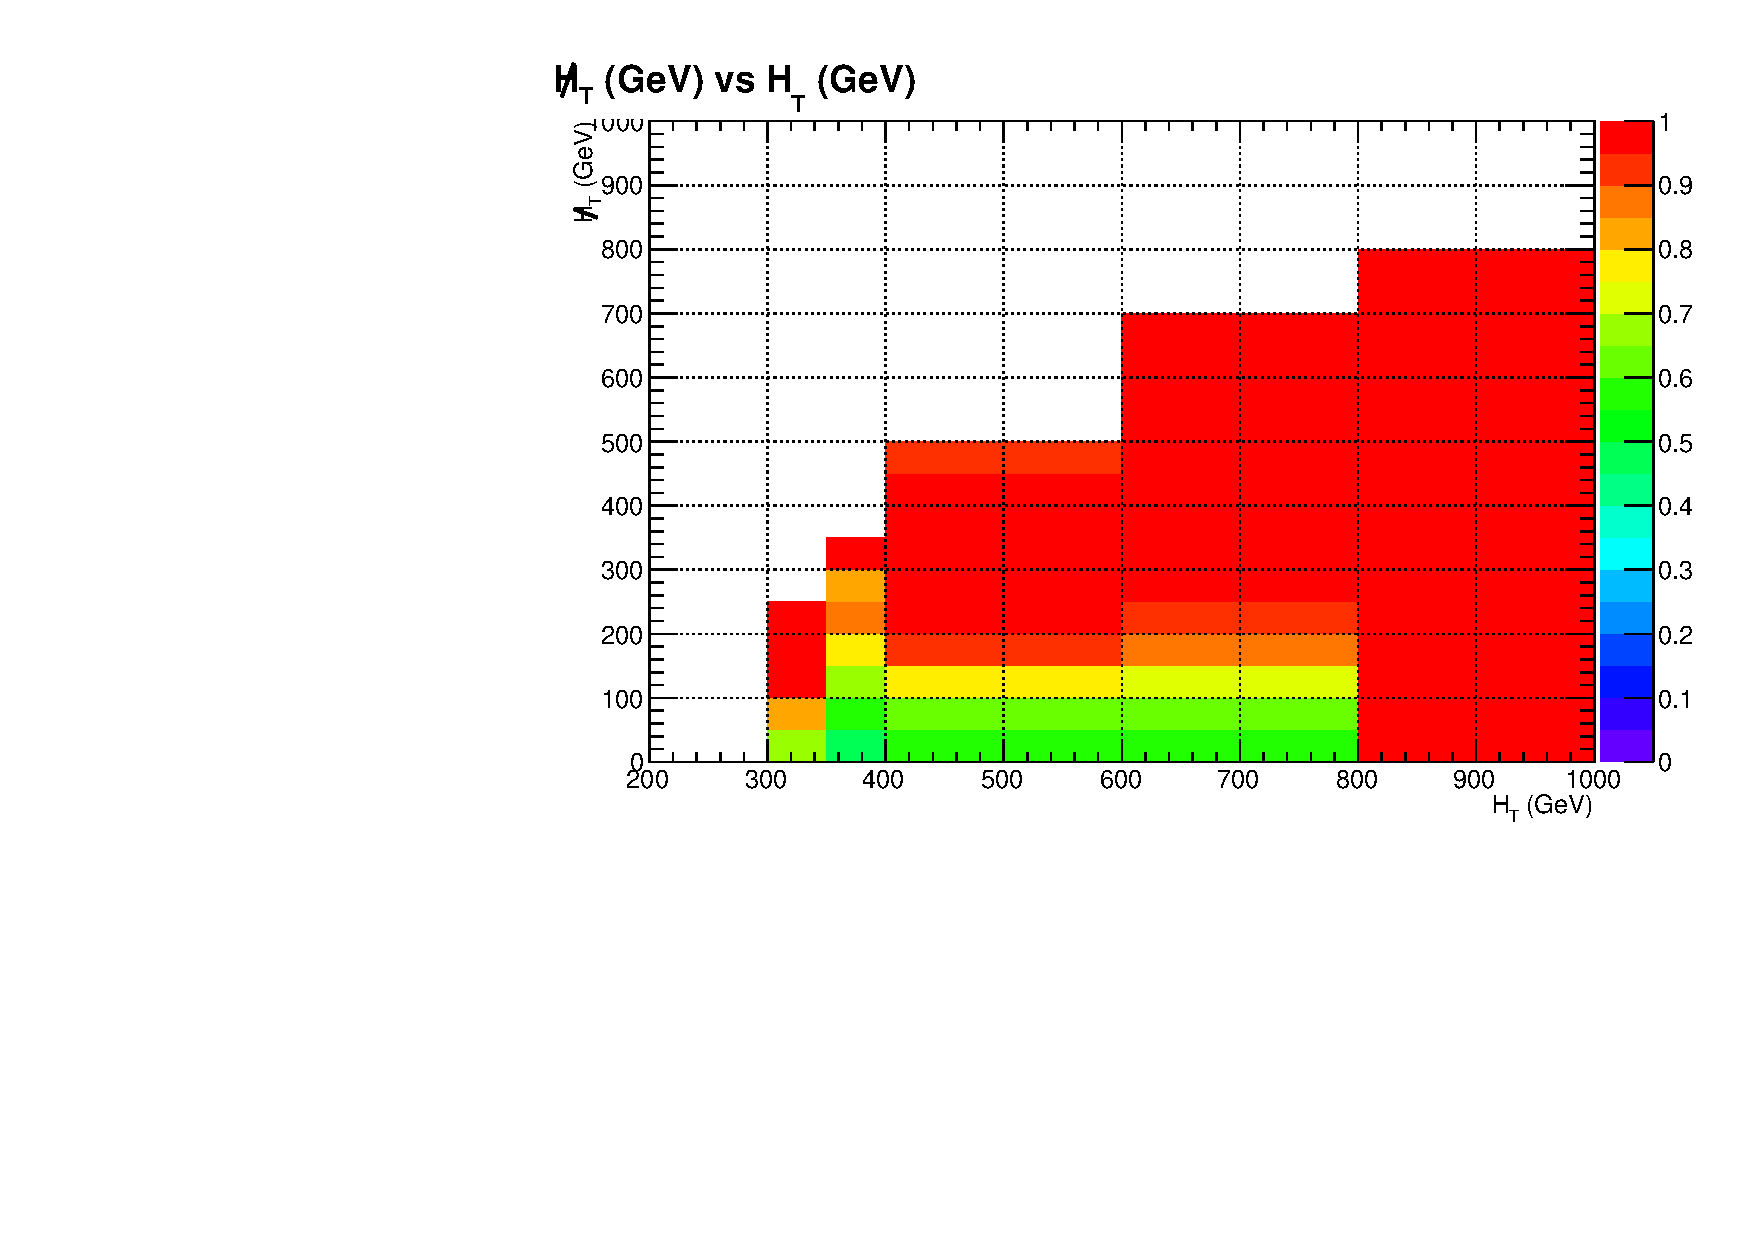
\includegraphics[width=0.5\textwidth]{figures/Trigger/ge5j_ht_vs_mht_Cumul.pdf}} \\
    \caption{
Cumulative trigger efficiency for the {\verb!T1tttt}(1200,800) model after signal selection in the \alphat-\scalht and \mht-\scalht planes for representative analysis jet multiplicity bins.}
    \label{fig:T1ttt_Trigger_Efficiency}
  \end{center} 
\end{figure}







% Control region triggers
\subsection{Control samples}
Prescaled $\scalht$ triggers shown in Table~\ref{tab:2015_Hadronic_Control_Triggers} are utilised in the selection of events for the hadronic control region. These share the same Level-1 seeds and $\scalht$ threshold of the signal triggers and are similarly each mapped to a unique offline bin. 


% TABLE: Hadronic control region
%----------------------------------------------------------------------
\begin{table}[h!]
\topcaption{Hadronic control triggers. }
\footnotesize
\centering
\begin{tabular}{c|cc} 
\hline
\hline
HLT path & \multicolumn{2}{c}{Prescale} \\
         & $\lumi=1.4\times10^{34}$  & $\lumi=7\times10^{33}$     \\
\hline
\verb!HLT_PFHT200! & 12600 & 6300 \\
\verb!HLT_PFHT250! & 8400  & 4200 \\
\verb!HLT_PFHT300! & 4200  & 2100 \\
\verb!HLT_PFHT350! & 700   & 350  \\
\verb!HLT_PFHT400! & 1400  & 700  \\
\hline
\hline

\end{tabular}
\label{tab:2015_Hadronic_Control_Triggers}
\end{table}




The non-hadronic control regions will be seeded by the lowest-threshold unprescaled triggers of the given run scenario, with \verb!HLT_Ele27_eta2p1_WP75_Gsf! seeding the electron control region ($e$, $ee$), \verb!HLT_IsoMu20_eta2p1! the muon control region ($\mu$, $\mu\mu$) and \verb!HLT_Photon175! the photon control region.





\subsection{Low-$\scalht$ Level-1 seeds}

Some models of new physics, such as supersymmetric compressed spectrum models, are challenging to select at the trigger level due to low-hadronic energy visible in the final state. Sensitivity to such models require low trigger thresholds which is difficult to achieve without incurring a large increase in the Level-1 trigger rate. New Level-1 seeds which enable low thresholds to be utilised by actively vetoing QCD event topologies have been studied and are shown to have higher efficiencies for such models than can be achieved with the current Level-1 menu.

The $\Delta\phi(j_{1}^{L1},j_{2}^{L1})$ seed exploits the typical dijet topologies exhibited in QCD dijet production by vetoing events where the azimuthal separation of the leading jets exceeds eight calorimeter regions, corresponding to a veto of: $\Delta\phi(j_{1}^{L1},j_{2}^{L1}) \ge 160^{\circ}$, where a jet threshold of $\pt > 32$ GeV is imposed on the second jet. This enables a much lower threshold on the $\scalht$-leg to be achieved, with a small increase in other thresholds in the menu, enabling for example the rate neutral trigger: \verb!L1_DoubleJetC32_WdPhi7_HTT125! to be utilised.

An alternate $\mht/\scalht$ 'reduced-MHT' seed exploits the correlation in missing hadronic energy and visible hadronic energy typical of decays with genuine $\met$ and the decorrelation of these quantities for QCD with fake-$\met$ by requiring a minimum $\mht/\scalht$ ratio. This again enables triggers with a significant reduction in the threshold on the $\scalht$-leg, for example with the rate neutral trigger: \verb!L1_HTT125_rHTM0p3!.

The logical disjunction of these two seeds can further improve signal efficiency whilst maintaining an effective suppression of QCD events by increasing acceptance to additional topolgies. ISR-dominated final states for instance typically have large $\mht/\scalht$ but may fail the $\Delta\phi(j_{1}^{L1},j_{2}^{L1})$ selection, where as events with high jet multiplicities typically have high $\Delta\phi(j_{1}^{L1},j_{2}^{L1})$ but may fail the $\mht/\scalht$ threshold due to the breakdown in $\mht/\scalht$ at high jet multiplicities. Combined these seeds allow even smaller thresholds to be used on the $\scalht$-leg without loss of efficiency to ISR-dominated or high jet multiplicity events, for example with the trigger:\\ \verb!L1_HTT110_rHTM0p6_rHTM0p0_WdPhi6!.


\subsubsection{Implementation and performance of low-$\scalht$ Level-1 seeds}

The new trigger seeds can be implemented in the trigger hardware by repurposing the bits currently utilised for $\mht$ and $\phi({\mht})$ trigger primitives with the new $\mht/\scalht$ and $\Delta\phi(j_{1}^{L1},j_{2}^{L1})$ primitives respectively. These changes have been discussed with trigger experts and are deemed to be relatively simple to implement in the calorimeter trigger firmware and will have little impact on the operation global trigger. The latest version of the Level-1 trigger emulator currently has the \verb!L1_DoubleJetC32_WdPhi7_HTT125!, \verb!L1_HTT125_rHTM0p3! and \\ \verb!L1_HTT110_rHTM0p6_rHTM0p0_WdPhi6! low-$\scalht$ trigger primitives implemented, enabling a wider study within the collaboration.

The performance after the full offline selection of the low-$\scalht$ Level-1 seeds was studied for a range of signal models in the lowest $\scalht$ and $\njet$ analysis bins which are predominantly populated by compressed models. Performance was measured relative to the current PU40bx25 Level-1 hadronic menu, {\verb!HTT175! \verb!OR! \verb!DoubleJetC100! \verb!OR! \verb!QuadJetC60! \verb!OR! \verb!ETM70!}, with the rate equivalent low-$\scalht$ menues defined as: Low-$\scalht$ seed {\verb!OR! \verb!HTT200! \verb!OR! \verb!DoubleJetC120! \verb!OR! \verb!QuadJetC60! \verb!OR! \verb!ETM70!}. The efficiencies of the proposed menues for $\njet = 2$ and $\njet = 3$, shown in Table~\ref{tab:LowHT_Seed_Signal_2Jet} and Table~\ref{tab:LowHT_Seed_Signal_3Jet} respectively, show significant improvements in trigger efficiency utilising the low-$\scalht$ seeds with respect to the current hadronic menu and similar performance to what could be obtained by reducing the $\met$ threshold without the additional 3 kHz Level-1 trigger rate this would incur.


% TABLE : Low-HT seed efficiencies - NJet = 2
%----------------------------------------------------------------------
\begin{table}[h!]
\topcaption{Trigger efficiency for $\njet = 2$, $200 < \scalht \le 300$ analysis bin and corresponding rate of the current Level-1 hadronic menu and proposed low-$\scalht$ trigger menues for a range of compressed signal models.} %sparticle and LSP masses represented by the first and second bracketed term respectively.}
\footnotesize
\centering
\begin{tabular}{cccccc} 
\hline
\hline
  Signal model & Hadronic menu & $\Delta\phi(j_{1}^{L1},j_{2}^{L1})$ & $\mht/\scalht$ &$\Delta\phi(j_{1}^{L1},j_{2}^{L1})$ \verb!OR! $\mht/\scalht$ & Hadronic menu \verb!OR ETM60! \\
\hline
  T2cc(250, 210)   & 0.60 & 0.86 & 0.91 & 0.94 & 0.95 \\
  T2qq(400, 400)   & 0.63 & 0.82 & 0.88 & 0.95 & 0.94 \\
  T2tt(300, 200)   & 0.53 & 0.91 & 0.95 & 0.99 & 0.96 \\
\hline
  Menu rate (kHz) & 15   & 15   & 15   & 15   & 19   \\
\hline
\hline
\end{tabular}
\label{tab:LowHT_Seed_Signal_2Jet}
\end{table}

% TABLE : Low-HT seed efficiencies - NJet = 3
%----------------------------------------------------------------------
\begin{table}[h!]
\topcaption{Trigger efficiency for $\njet = 3$, $200 < \scalht \le 300$ analysis bin and corresponding rate of the current Level-1 hadronic menu and proposed low-$\scalht$ trigger menues for a range of compressed signal models.} %sparticle and LSP masses represented by the first and second bracketed term respectively.}
\footnotesize
\centering
\begin{tabular}{cccccc} 
\hline
\hline
  Signal model & Hadronic menu & $\Delta\phi(j_{1}^{L1},j_{2}^{L1})$ & $\mht/\scalht$ &$\Delta\phi(j_{1}^{L1},j_{2}^{L1})$ \verb!OR! $\mht/\scalht$ & Hadronic menu \verb!OR ETM60! \\
\hline
  T2cc(250, 210)   & 0.45 & 0.74 & 0.74 & 0.83 & 0.94 \\
  T2qq(400, 400)   & 0.46 & 0.88 & 0.88 & 0.93 & 0.92 \\
  T2tt(300, 200)   & 0.41 & 0.76 & 0.83 & 0.84 & 0.86 \\
\hline
  Menu rate (kHz) & 15   & 15   & 15   & 15   & 19   \\
\hline
\hline
\end{tabular}
\label{tab:LowHT_Seed_Signal_3Jet}
\end{table}



%%____________________________________________________________________________||
